\section{Desarrollo de una aplicación}

% Escoger una aplicación real y describir como se hace en cada etapa. Las etapas que debemos abordar son:
%       Adquisición de las imágenes o video
%       Preprocesamiento
%       Segmentación
%       Extracción de características
%       Clasificación

% 3. Como ejemplo: Sistema de CV: Reconocimiento de matrículas de coche
% Módulos (habría que desarrollarlos):
% - Adquisición: Cámara (y características). No dependiente de la luminosidad: Infraroja. Múltiples para captar varios ángulos
% - Preprocesamiento: Eliminación de ruido, añadiendo contraste. Cálculo de límites de los objetos
% - Segmentación: El coche del fondo, la matrícula del coche, cada carácter de la matrícula
% - Extracción de características (a no ser que se use convolución): Histogramas de orientación de gradiente, entropía, información de las fronteras...
% - Clasificación: SVC, KMeans, RNN, CNN (extraen características a la vez que clasifican). Supervisado, no supervisado...

% Los módulos pueden estar conectados a una base de conocimiento (con el dominio del problema) que indique lo que debe hacer cada uno.

% \begin{figure}[h]
%   \centerfloat
%   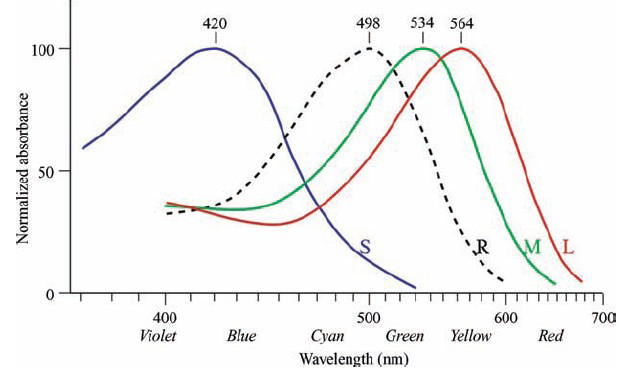
\includegraphics[width=0.75\textwidth]{img/conos.png}
%   % \caption{Relación intermediación-vector propio en escala logarítmica.}
% \end{figure}